\subsection{Training}
We optimize the hyper-parameters of kernels by maximizing the marginal likelihood marginalized over function values f at the whole locations X. We use the publicly available python package sklearn\cite{scikit-learn} to reconstruct distance modulus as a function of redshift. The results are plotted in \eqref{fig:gp_re}. The posterior samples drawn from kernel is shown in \eqref{fig:posterior_pantheon} .In the range where data points are sparse, the uncertainty of the reconstructed function is large. While training GP numerical issues are common to occur, hence we set $\alpha=0.3$ and standardize the distance modulus before training. We also restart optimizer 100 times, parameters sampled log-uniform randomly from the space of allowed range.

\begin{figure}[h]
	\centering
	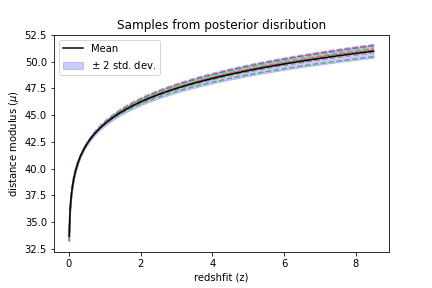
\includegraphics[width=\textwidth]{pantheon/gp/02_Sample_posterior_distibutions.png}
	\caption{Posterior samples drawn from GP}
	\label{fig:posterior_pantheon}
\end{figure}

The error bars with predictions are shown below
\begin{figure}[h]
	\centering
	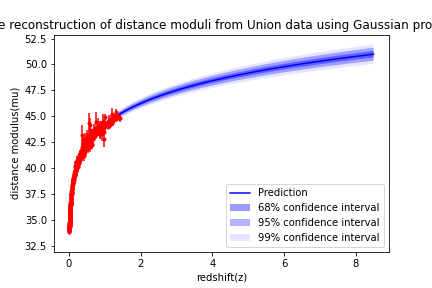
\includegraphics[width=\textwidth]{pantheon/gp/03_Reconstruction_GP.png}
	\caption{The reconstruction of distance moduli from Pantheon data set using GP. The red dots with $1\sigma$ error bars are the Pantheon data points. The light-blue dots are the central values of reconstruction. The shaded regions are the $1\sigma$, $2\sigma$ and $3\sigma$ uncertainties.}
	\label{fig:gp_re}
\end{figure}

Log Marginal Likelihood = -20.3

The coefficient of determination $R^2$ = 0.9951